\subsubsection{Navadne krivulje}
Novejši postopki so olajšali izdelavo krivulj. Z CNC rezkanjem se 
lahko krivulja zelo hitro in natančno izdela, potrebno pa je 
narediti posebno vpetje, saj primež ni primeren za to. Možna je 
tudi izdelava z žično erozijo, kjer vpetje ni problem, je pa dražji
postopek izdelave. 

Najbolj pogosto se izdelujejo iz jekla CK45 (1.1191), ki vsebuje 
0.45 \% C, 0.65 \% Mn, 0.035 \% P in manj kot 0.035 \% S in ima natezno trdnost okoli 725 MPa.

Pred CNC stroji so krivulje izdelovali ročno na rezkalnih strojih 
in z brusilkami, ali pa na klasični stružnici z vgrajeno vrtalno glavo. 

Najprej se je ročno izrisala krivulja in se prenesla na surovec. 
Če je bil surovec veliko večji od načrtovane krivulje, so po 
zunanji konturi zvrtali luknje tako, da so se približno 1-2mm 
prekrivale. Potem se je krivulja izbila iz prvotnega surovca, 
se vpela v primež in so jo z brusilko izbrusili v končno obliko. 
Za tem, če je bilo potrebno izdelati točen vzpon krivulje, je to 
možno porezkat na klasični stružnici z vgrajeno vrtalno glavo in 
delilnim aparatom. 

Spodaj, na sliki \ref{ploscate_krivulje} je prikazanih nekaj primerov
izdelanih ploščatih krivulj.

\begin{figure}[H]
    \begin{center}
        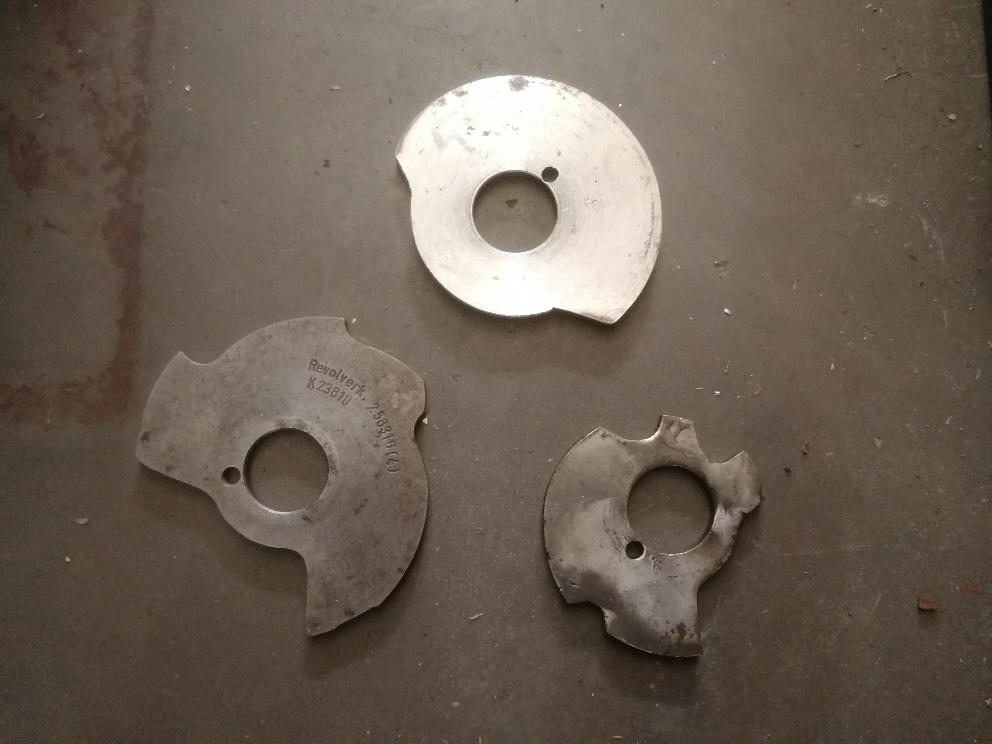
\includegraphics[width=13cm]{ploscate_krivulje.jpg}
        \caption{Ploščata krivulja
        \cite{lasten}}   
        \label{ploscate_krivulje}
    \end{center}
\end{figure}
\newpage
\subsubsection{Preračun navadnih krivulj}
\label{izracun_krivulj}
Primer: imamo obdelovanec premera 12 mm, ki se vrti z hitrostjo \( \frac{obr}{min} \)
in časom enega cikla 30 s. Hočemo ga odrezat z odreznim nožem z pomikom 0.04 \( \frac{mm}{obr} \)
(Da stvar poenostavimo sem že izbral željen pomik na obrat, namesto da bi ga 
izračunal iz rezalne hitrosti in premera)

Zaradi varnosti, bomo določili, da nož začne z delovnim gibom 
na $\phi13$ in konča na $\phi-1$. To pomeni, da bo potoval 7 mm, ker 
imamo simetrično obdelovanje. 

Iz tega izračunamo število vrtljajev N, potrebnih za ta pomik po spodnji enačbi \ref{st_vrtljajev}:

\begin{equation}
    \label{st_vrtljajev}
    \begin{split}
        N &= \frac{l}{f} \\
        N &= \frac{7mm}{0.04\frac{mm}{obr}}
    \end{split}
\end{equation}

Dobimo, da se bo glavno vreteno zavrtelo za 175 vrtljajev v tem 
pomiku. Iz tega podatka po sorazmerju izračunamo čas, potreben 
za hod po enačbi \ref{cas_za_hod}.

\begin{equation}
    \label{cas_za_hod}
    \begin{split}
        \frac{2000vrt}{60s} &= \frac{175vrt}{t} \\
        t &= \frac{60s * 175vrt}{2000vrt} \\
        t &= 5.25s
    \end{split}
\end{equation}
 
V 5.25 s se bo izvedel odrez. Z tem podatkom nato z enačbo \ref{kot_krivulje} izračunamo 
kolikšen kot krivulje mora obsegati vzpon, da bomo dosegli željen pomik.

\begin{equation}
    \label{kot_krivulje}
    \begin{split}
        \alpha &= \frac{360\degree}{T} * t \\
        \alpha &= \frac{360\degree}{30s} * 5.25s \\
        \alpha &= 63\degree
    \end{split}    
\end{equation}

Če imamo razmerje med vzvodi vodila in nožem 1:1, potem se more krivulja v 63° vzpet za 7 mm.
Zdaj imamo dve možnosti:
\begin{itemize}
    \item Izdelamo krivuljo po meri
    \item Izberemo najbližjo standardno krivuljo po raznih katalogih ali zalogi.
\end{itemize}

\newpage
\subsubsection{Bobnaste krivulje}
Sodobna izdelava bobnastih krivulj poteka na CNC rezkalnih strojih 
z 4. (C) osjo. Pred tem, pa so bobnaste krivulje večinoma delali v
odsekih in jih z tem ločili na hitre in delovne gibe in je bilo z tem
mogoče lažje in bolj natančno nastavljati zamike krivulj.
Možno je tudi, da se obrabljena krivulja enostavno zamenja brez
večjega zastoja. Po izdelavi se zakalijo na približno 50-60 HRC.

Na spodnji sliki \ref{bobnaste_krivulje} je prikazan primer 
bobnaste krivulje.

\begin{figure}[H]
    \begin{center}
        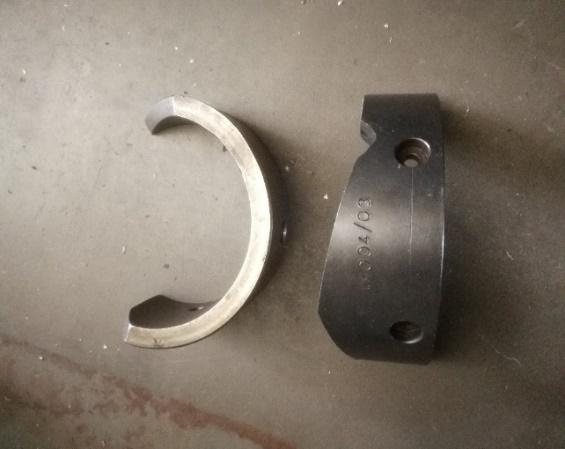
\includegraphics[width=\linewidth]{bobnasta_krivulja.jpg}
        \caption{Bobnasta krivulja
        \cite{lasten}}   
        \label{bobnaste_krivulje}
    \end{center}
\end{figure}

\newpage
\subsubsection{Kaljenje}
Po izdelavi se krivulje kalijo, da zmanjšamo obrabo. Kaljenje 
je toplotna izdelava s katerim dosežemo utrjeno površino in jedro. 
Obdelava je sestavljena z segrevanjem, zadrževanjem na temperaturi 
kaljenja, hitrim ohlajanjem in popuščanjem, kot je vidno na spodnji
sliki \ref{diagram_kaljenja}.

\begin{figure}[H]
    \begin{center}
        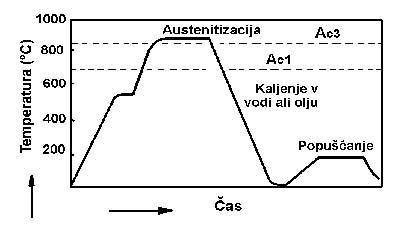
\includegraphics[width=\linewidth]{diagram_kaljenja.jpg}
        \caption{Diagram kaljenja z popuščanjem
        \cite{diagram_kaljenja}}
        \label{diagram_kaljenja}
    \end{center}
\end{figure}

Kalimo lahko na naslednje načine:
\begin{itemize}
    \item Kaljenje v pečeh
    \item Induktivno Kaljenje
    \item Plamensko kaljenje
\end{itemize}

Na sliki \ref{induktivno_kaljenje} je prikazan primer induktivnega 
segrevanja obdelovanca med bakrenimi obroči.

\begin{figure}[H]
    \begin{center}
        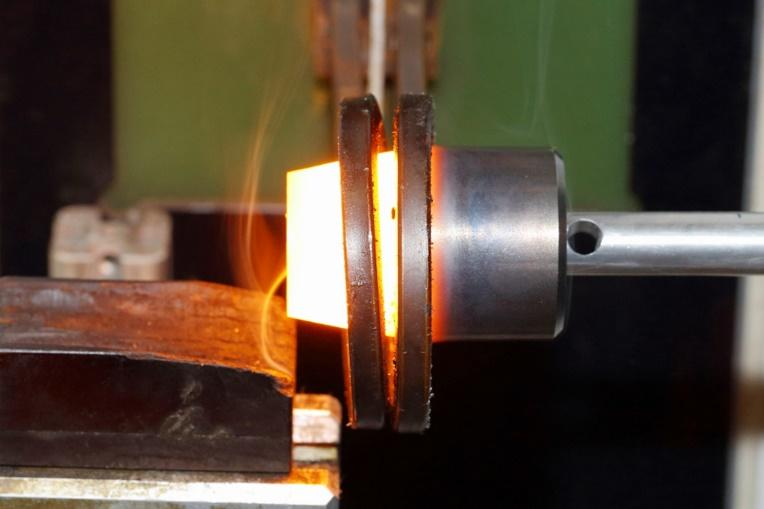
\includegraphics[width=\linewidth]{induktivno_kaljenje.jpg}
        \caption{Slika induktivnega kaljenja
        \cite{lasten}}
        \label{induktivno_kaljenje}
    \end{center}
\end{figure}

Kaljenje v pečeh in induktivno kaljenje je v večji meri uporabno 
za večje količine kosov. Omogoča namreč hitro in natančno kaljenje,
saj so sodobne peči elektronsko krmiljene in opremljene z raznimi senzorji.

Plamensko kaljenje se pa uporablja za manjše količine ali za 
posamične kose, kateri ne potrebujejo natančne trdote. Za 
segrevanje se uporablja plamenski gorilnik, z katerim segrejemo 
material do določene barve in ga nato ohladimo v vodi ali v olju.

Temperature kaljenja so odvisne od jekla in njegovih legirnih 
elementov. Segajo od 700 °C do 900 °C, temperature popuščanja 
pa od 200 °C do 500 °C. Močnejše legirana jekla je potrebno 
segrevati počasi do okolice 400 °C do 500 °C, da postane jeklo 
duktilno nato ga lahko segrevamo hitreje. 

Trajanje kaljenja je odvisno od debeline sten izdelka, njegove toplotne 
prevodnosti in sredstva v katerem ga segrevamo. Pri prekratkem 
segrevanju se notranjost predmetov ne segreje do zahtevane 
temperature, kar privede do nepopolnega postopka obdelave. Pri 
predolgem segrevanju pa se lahko pojavlja grobozrnata struktura 
in delno razogličenje jekla.

\newpage